\documentclass[12pt]{article}
\usepackage[letterpaper,top=0.8in,bottom=0.8in,left=0.5in,right=0.5in,
            headheight=15pt,headsep=0.25in,footskip=0.4in]{geometry}
\usepackage[T1]{fontenc}
\usepackage{helvet}
\renewcommand{\familydefault}{\sfdefault}
\usepackage{tikz}
\usetikzlibrary{shapes.geometric}
\usepackage{fancyhdr}
\usepackage{xcolor}

\definecolor{redtint}{RGB}{248,180,172}
\definecolor{bluetint}{RGB}{110,150,215}
\definecolor{redctr}{RGB}{235,95,85}
\definecolor{bluectr}{RGB}{30,70,160}
\definecolor{gridline}{RGB}{60,60,60}
\definecolor{writeline}{RGB}{185,185,185}

\pagestyle{fancy}
\fancyhf{}
\lhead{Week NN / Hex / Grades K--1}
\lfoot{Bellingham Math Circle / Week NN / HEX-K-v1}
\rfoot{\thepage}
\renewcommand{\headrulewidth}{0pt}
\setlength{\parindent}{0pt}
\setlength{\parskip}{0pt}
\newcommand{\prob}[1]{\textbf{Problem #1:}}
\newsavebox{\landbox}
\begin{document}
\large\raggedright
\begin{minipage}[c]{0.56\textwidth}\raggedright Red and Blue take turns putting a counter of their own color on an empty hexagon. Red wins by joining the two red edges with a chain of red hexagons. Blue wins by joining the two blue edges with a chain of blue hexagons. Each hexagon in a chain shares a side with the next one.\end{minipage}\hfill\begin{minipage}[c]{0.38\textwidth}\centering 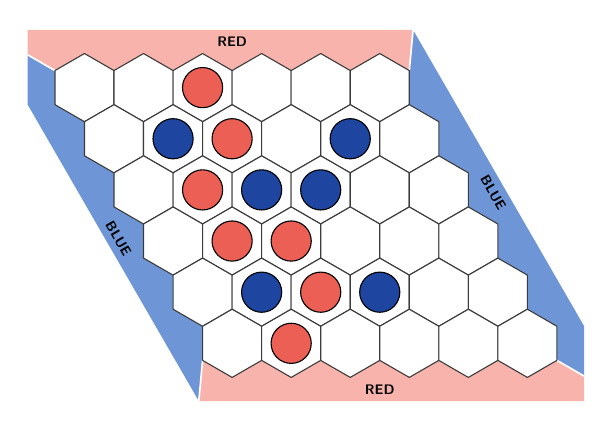
\begin{tikzpicture}[x=1.0mm,y=1.0mm,line join=round]
\begin{scope}
\clip (-7.214,-39.806) rectangle (63.464,7.330);
\fill[redtint] (-3.750,2.165) -- (0.000,4.330) -- (3.750,2.165) -- (7.500,4.330) -- (11.250,2.165) -- (15.000,4.330) -- (18.750,2.165) -- (22.500,4.330) -- (26.250,2.165) -- (30.000,4.330) -- (33.750,2.165) -- (37.500,4.330) -- (41.250,2.165) -- (41.732,7.330) -- (-12.696,7.330) -- cycle;
\fill[redtint] (60.000,-34.641) -- (56.250,-36.806) -- (52.500,-34.641) -- (48.750,-36.806) -- (45.000,-34.641) -- (41.250,-36.806) -- (37.500,-34.641) -- (33.750,-36.806) -- (30.000,-34.641) -- (26.250,-36.806) -- (22.500,-34.641) -- (18.750,-36.806) -- (15.000,-34.641) -- (14.518,-39.806) -- (68.946,-39.806) -- cycle;
\fill[bluetint] (15.000,-34.641) -- (15.000,-30.311) -- (11.250,-28.146) -- (11.250,-23.816) -- (7.500,-21.651) -- (7.500,-17.321) -- (3.750,-15.155) -- (3.750,-10.825) -- (0.000,-8.660) -- (-0.000,-4.330) -- (-3.750,-2.165) -- (-3.750,2.165) -- (-12.696,7.330) -- (14.518,-39.806) -- cycle;
\fill[bluetint] (41.250,2.165) -- (41.250,-2.165) -- (45.000,-4.330) -- (45.000,-8.660) -- (48.750,-10.825) -- (48.750,-15.155) -- (52.500,-17.321) -- (52.500,-21.651) -- (56.250,-23.816) -- (56.250,-28.146) -- (60.000,-30.311) -- (60.000,-34.641) -- (68.946,-39.806) -- (41.732,7.330) -- cycle;
\draw[white,line width=0.6pt] (-3.750,2.165) -- (-12.696,7.330);
\draw[white,line width=0.6pt] (41.250,2.165) -- (41.732,7.330);
\draw[white,line width=0.6pt] (60.000,-34.641) -- (68.946,-39.806);
\draw[white,line width=0.6pt] (15.000,-34.641) -- (14.518,-39.806);
\end{scope}
\node[font=\tiny\bfseries,text=black] at (18.750,5.830) {RED};
\node[font=\tiny\bfseries,text=black] at (37.500,-38.306) {RED};
\node[font=\tiny\bfseries,text=black,rotate=-60] at (4.326,-19.153) {BLUE};
\node[font=\tiny\bfseries,text=black,rotate=-60] at (51.924,-13.323) {BLUE};
\filldraw[fill=white,draw=gridline,line width=0.4pt] (3.750,2.165) -- (0.000,4.330) -- (-3.750,2.165) -- (-3.750,-2.165) -- (-0.000,-4.330) -- (3.750,-2.165) -- cycle;
\filldraw[fill=white,draw=gridline,line width=0.4pt] (11.250,2.165) -- (7.500,4.330) -- (3.750,2.165) -- (3.750,-2.165) -- (7.500,-4.330) -- (11.250,-2.165) -- cycle;
\filldraw[fill=white,draw=gridline,line width=0.4pt] (18.750,2.165) -- (15.000,4.330) -- (11.250,2.165) -- (11.250,-2.165) -- (15.000,-4.330) -- (18.750,-2.165) -- cycle;
\filldraw[fill=white,draw=gridline,line width=0.4pt] (26.250,2.165) -- (22.500,4.330) -- (18.750,2.165) -- (18.750,-2.165) -- (22.500,-4.330) -- (26.250,-2.165) -- cycle;
\filldraw[fill=white,draw=gridline,line width=0.4pt] (33.750,2.165) -- (30.000,4.330) -- (26.250,2.165) -- (26.250,-2.165) -- (30.000,-4.330) -- (33.750,-2.165) -- cycle;
\filldraw[fill=white,draw=gridline,line width=0.4pt] (41.250,2.165) -- (37.500,4.330) -- (33.750,2.165) -- (33.750,-2.165) -- (37.500,-4.330) -- (41.250,-2.165) -- cycle;
\filldraw[fill=white,draw=gridline,line width=0.4pt] (7.500,-4.330) -- (3.750,-2.165) -- (-0.000,-4.330) -- (0.000,-8.660) -- (3.750,-10.825) -- (7.500,-8.660) -- cycle;
\filldraw[fill=white,draw=gridline,line width=0.4pt] (15.000,-4.330) -- (11.250,-2.165) -- (7.500,-4.330) -- (7.500,-8.660) -- (11.250,-10.825) -- (15.000,-8.660) -- cycle;
\filldraw[fill=white,draw=gridline,line width=0.4pt] (22.500,-4.330) -- (18.750,-2.165) -- (15.000,-4.330) -- (15.000,-8.660) -- (18.750,-10.825) -- (22.500,-8.660) -- cycle;
\filldraw[fill=white,draw=gridline,line width=0.4pt] (30.000,-4.330) -- (26.250,-2.165) -- (22.500,-4.330) -- (22.500,-8.660) -- (26.250,-10.825) -- (30.000,-8.660) -- cycle;
\filldraw[fill=white,draw=gridline,line width=0.4pt] (37.500,-4.330) -- (33.750,-2.165) -- (30.000,-4.330) -- (30.000,-8.660) -- (33.750,-10.825) -- (37.500,-8.660) -- cycle;
\filldraw[fill=white,draw=gridline,line width=0.4pt] (45.000,-4.330) -- (41.250,-2.165) -- (37.500,-4.330) -- (37.500,-8.660) -- (41.250,-10.825) -- (45.000,-8.660) -- cycle;
\filldraw[fill=white,draw=gridline,line width=0.4pt] (11.250,-10.825) -- (7.500,-8.660) -- (3.750,-10.825) -- (3.750,-15.155) -- (7.500,-17.321) -- (11.250,-15.155) -- cycle;
\filldraw[fill=white,draw=gridline,line width=0.4pt] (18.750,-10.825) -- (15.000,-8.660) -- (11.250,-10.825) -- (11.250,-15.155) -- (15.000,-17.321) -- (18.750,-15.155) -- cycle;
\filldraw[fill=white,draw=gridline,line width=0.4pt] (26.250,-10.825) -- (22.500,-8.660) -- (18.750,-10.825) -- (18.750,-15.155) -- (22.500,-17.321) -- (26.250,-15.155) -- cycle;
\filldraw[fill=white,draw=gridline,line width=0.4pt] (33.750,-10.825) -- (30.000,-8.660) -- (26.250,-10.825) -- (26.250,-15.155) -- (30.000,-17.321) -- (33.750,-15.155) -- cycle;
\filldraw[fill=white,draw=gridline,line width=0.4pt] (41.250,-10.825) -- (37.500,-8.660) -- (33.750,-10.825) -- (33.750,-15.155) -- (37.500,-17.321) -- (41.250,-15.155) -- cycle;
\filldraw[fill=white,draw=gridline,line width=0.4pt] (48.750,-10.825) -- (45.000,-8.660) -- (41.250,-10.825) -- (41.250,-15.155) -- (45.000,-17.321) -- (48.750,-15.155) -- cycle;
\filldraw[fill=white,draw=gridline,line width=0.4pt] (15.000,-17.321) -- (11.250,-15.155) -- (7.500,-17.321) -- (7.500,-21.651) -- (11.250,-23.816) -- (15.000,-21.651) -- cycle;
\filldraw[fill=white,draw=gridline,line width=0.4pt] (22.500,-17.321) -- (18.750,-15.155) -- (15.000,-17.321) -- (15.000,-21.651) -- (18.750,-23.816) -- (22.500,-21.651) -- cycle;
\filldraw[fill=white,draw=gridline,line width=0.4pt] (30.000,-17.321) -- (26.250,-15.155) -- (22.500,-17.321) -- (22.500,-21.651) -- (26.250,-23.816) -- (30.000,-21.651) -- cycle;
\filldraw[fill=white,draw=gridline,line width=0.4pt] (37.500,-17.321) -- (33.750,-15.155) -- (30.000,-17.321) -- (30.000,-21.651) -- (33.750,-23.816) -- (37.500,-21.651) -- cycle;
\filldraw[fill=white,draw=gridline,line width=0.4pt] (45.000,-17.321) -- (41.250,-15.155) -- (37.500,-17.321) -- (37.500,-21.651) -- (41.250,-23.816) -- (45.000,-21.651) -- cycle;
\filldraw[fill=white,draw=gridline,line width=0.4pt] (52.500,-17.321) -- (48.750,-15.155) -- (45.000,-17.321) -- (45.000,-21.651) -- (48.750,-23.816) -- (52.500,-21.651) -- cycle;
\filldraw[fill=white,draw=gridline,line width=0.4pt] (18.750,-23.816) -- (15.000,-21.651) -- (11.250,-23.816) -- (11.250,-28.146) -- (15.000,-30.311) -- (18.750,-28.146) -- cycle;
\filldraw[fill=white,draw=gridline,line width=0.4pt] (26.250,-23.816) -- (22.500,-21.651) -- (18.750,-23.816) -- (18.750,-28.146) -- (22.500,-30.311) -- (26.250,-28.146) -- cycle;
\filldraw[fill=white,draw=gridline,line width=0.4pt] (33.750,-23.816) -- (30.000,-21.651) -- (26.250,-23.816) -- (26.250,-28.146) -- (30.000,-30.311) -- (33.750,-28.146) -- cycle;
\filldraw[fill=white,draw=gridline,line width=0.4pt] (41.250,-23.816) -- (37.500,-21.651) -- (33.750,-23.816) -- (33.750,-28.146) -- (37.500,-30.311) -- (41.250,-28.146) -- cycle;
\filldraw[fill=white,draw=gridline,line width=0.4pt] (48.750,-23.816) -- (45.000,-21.651) -- (41.250,-23.816) -- (41.250,-28.146) -- (45.000,-30.311) -- (48.750,-28.146) -- cycle;
\filldraw[fill=white,draw=gridline,line width=0.4pt] (56.250,-23.816) -- (52.500,-21.651) -- (48.750,-23.816) -- (48.750,-28.146) -- (52.500,-30.311) -- (56.250,-28.146) -- cycle;
\filldraw[fill=white,draw=gridline,line width=0.4pt] (22.500,-30.311) -- (18.750,-28.146) -- (15.000,-30.311) -- (15.000,-34.641) -- (18.750,-36.806) -- (22.500,-34.641) -- cycle;
\filldraw[fill=white,draw=gridline,line width=0.4pt] (30.000,-30.311) -- (26.250,-28.146) -- (22.500,-30.311) -- (22.500,-34.641) -- (26.250,-36.806) -- (30.000,-34.641) -- cycle;
\filldraw[fill=white,draw=gridline,line width=0.4pt] (37.500,-30.311) -- (33.750,-28.146) -- (30.000,-30.311) -- (30.000,-34.641) -- (33.750,-36.806) -- (37.500,-34.641) -- cycle;
\filldraw[fill=white,draw=gridline,line width=0.4pt] (45.000,-30.311) -- (41.250,-28.146) -- (37.500,-30.311) -- (37.500,-34.641) -- (41.250,-36.806) -- (45.000,-34.641) -- cycle;
\filldraw[fill=white,draw=gridline,line width=0.4pt] (52.500,-30.311) -- (48.750,-28.146) -- (45.000,-30.311) -- (45.000,-34.641) -- (48.750,-36.806) -- (52.500,-34.641) -- cycle;
\filldraw[fill=white,draw=gridline,line width=0.4pt] (60.000,-30.311) -- (56.250,-28.146) -- (52.500,-30.311) -- (52.500,-34.641) -- (56.250,-36.806) -- (60.000,-34.641) -- cycle;
\filldraw[fill=redctr,draw=black,line width=0.4pt] (15.000,0.000) circle (2.550);
\filldraw[fill=redctr,draw=black,line width=0.4pt] (18.750,-6.495) circle (2.550);
\filldraw[fill=redctr,draw=black,line width=0.4pt] (15.000,-12.990) circle (2.550);
\filldraw[fill=redctr,draw=black,line width=0.4pt] (18.750,-19.486) circle (2.550);
\filldraw[fill=redctr,draw=black,line width=0.4pt] (26.250,-19.486) circle (2.550);
\filldraw[fill=redctr,draw=black,line width=0.4pt] (30.000,-25.981) circle (2.550);
\filldraw[fill=redctr,draw=black,line width=0.4pt] (26.250,-32.476) circle (2.550);
\filldraw[fill=bluectr,draw=black,line width=0.4pt] (11.250,-6.495) circle (2.550);
\filldraw[fill=bluectr,draw=black,line width=0.4pt] (22.500,-12.990) circle (2.550);
\filldraw[fill=bluectr,draw=black,line width=0.4pt] (30.000,-12.990) circle (2.550);
\filldraw[fill=bluectr,draw=black,line width=0.4pt] (22.500,-25.981) circle (2.550);
\filldraw[fill=bluectr,draw=black,line width=0.4pt] (37.500,-25.981) circle (2.550);
\filldraw[fill=bluectr,draw=black,line width=0.4pt] (33.750,-6.495) circle (2.550);
\end{tikzpicture}\end{minipage}
\par\vspace{7mm}
\prob{1} Play Hex on this board. Take turns going first.
\begin{center}
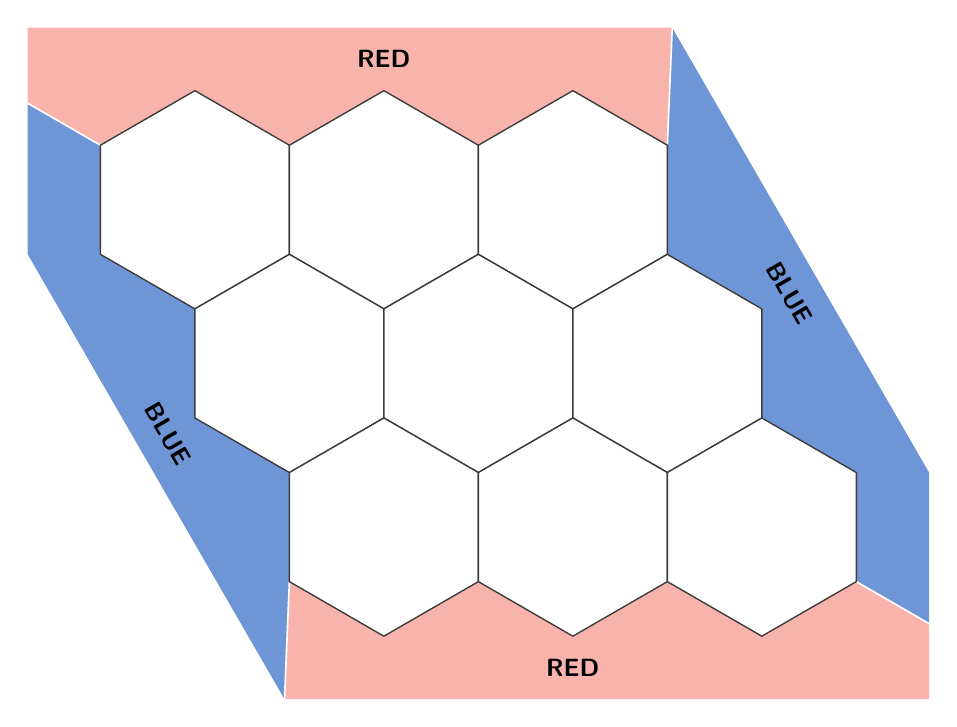
\begin{tikzpicture}[x=1.0mm,y=1.0mm,line join=round]
\begin{scope}
\clip (-21.238,-63.426) rectangle (93.238,21.856);
\fill[redtint] (-12.000,6.928) -- (0.000,13.856) -- (12.000,6.928) -- (24.000,13.856) -- (36.000,6.928) -- (48.000,13.856) -- (60.000,6.928) -- (60.619,21.856) -- (-37.856,21.856) -- cycle;
\fill[redtint] (84.000,-48.497) -- (72.000,-55.426) -- (60.000,-48.497) -- (48.000,-55.426) -- (36.000,-48.497) -- (24.000,-55.426) -- (12.000,-48.497) -- (11.381,-63.426) -- (109.856,-63.426) -- cycle;
\fill[bluetint] (12.000,-48.497) -- (12.000,-34.641) -- (0.000,-27.713) -- (-0.000,-13.856) -- (-12.000,-6.928) -- (-12.000,6.928) -- (-37.856,21.856) -- (11.381,-63.426) -- cycle;
\fill[bluetint] (60.000,6.928) -- (60.000,-6.928) -- (72.000,-13.856) -- (72.000,-27.713) -- (84.000,-34.641) -- (84.000,-48.497) -- (109.856,-63.426) -- (60.619,21.856) -- cycle;
\draw[white,line width=0.6pt] (-12.000,6.928) -- (-37.856,21.856);
\draw[white,line width=0.6pt] (60.000,6.928) -- (60.619,21.856);
\draw[white,line width=0.6pt] (84.000,-48.497) -- (109.856,-63.426);
\draw[white,line width=0.6pt] (12.000,-48.497) -- (11.381,-63.426);
\end{scope}
\node[font=\small\bfseries,text=black] at (24.000,17.856) {RED};
\node[font=\small\bfseries,text=black] at (48.000,-59.426) {RED};
\node[font=\small\bfseries,text=black,rotate=-60] at (-3.464,-29.713) {BLUE};
\node[font=\small\bfseries,text=black,rotate=-60] at (75.464,-11.856) {BLUE};
\filldraw[fill=white,draw=gridline,line width=0.5pt] (12.000,6.928) -- (0.000,13.856) -- (-12.000,6.928) -- (-12.000,-6.928) -- (-0.000,-13.856) -- (12.000,-6.928) -- cycle;
\filldraw[fill=white,draw=gridline,line width=0.5pt] (36.000,6.928) -- (24.000,13.856) -- (12.000,6.928) -- (12.000,-6.928) -- (24.000,-13.856) -- (36.000,-6.928) -- cycle;
\filldraw[fill=white,draw=gridline,line width=0.5pt] (60.000,6.928) -- (48.000,13.856) -- (36.000,6.928) -- (36.000,-6.928) -- (48.000,-13.856) -- (60.000,-6.928) -- cycle;
\filldraw[fill=white,draw=gridline,line width=0.5pt] (24.000,-13.856) -- (12.000,-6.928) -- (-0.000,-13.856) -- (0.000,-27.713) -- (12.000,-34.641) -- (24.000,-27.713) -- cycle;
\filldraw[fill=white,draw=gridline,line width=0.5pt] (48.000,-13.856) -- (36.000,-6.928) -- (24.000,-13.856) -- (24.000,-27.713) -- (36.000,-34.641) -- (48.000,-27.713) -- cycle;
\filldraw[fill=white,draw=gridline,line width=0.5pt] (72.000,-13.856) -- (60.000,-6.928) -- (48.000,-13.856) -- (48.000,-27.713) -- (60.000,-34.641) -- (72.000,-27.713) -- cycle;
\filldraw[fill=white,draw=gridline,line width=0.5pt] (36.000,-34.641) -- (24.000,-27.713) -- (12.000,-34.641) -- (12.000,-48.497) -- (24.000,-55.426) -- (36.000,-48.497) -- cycle;
\filldraw[fill=white,draw=gridline,line width=0.5pt] (60.000,-34.641) -- (48.000,-27.713) -- (36.000,-34.641) -- (36.000,-48.497) -- (48.000,-55.426) -- (60.000,-48.497) -- cycle;
\filldraw[fill=white,draw=gridline,line width=0.5pt] (84.000,-34.641) -- (72.000,-27.713) -- (60.000,-34.641) -- (60.000,-48.497) -- (72.000,-55.426) -- (84.000,-48.497) -- cycle;
\end{tikzpicture}
\end{center}

\clearpage
\prob{2} Can you put a red or a blue counter on every hexagon so that nobody wins?
\begin{center}
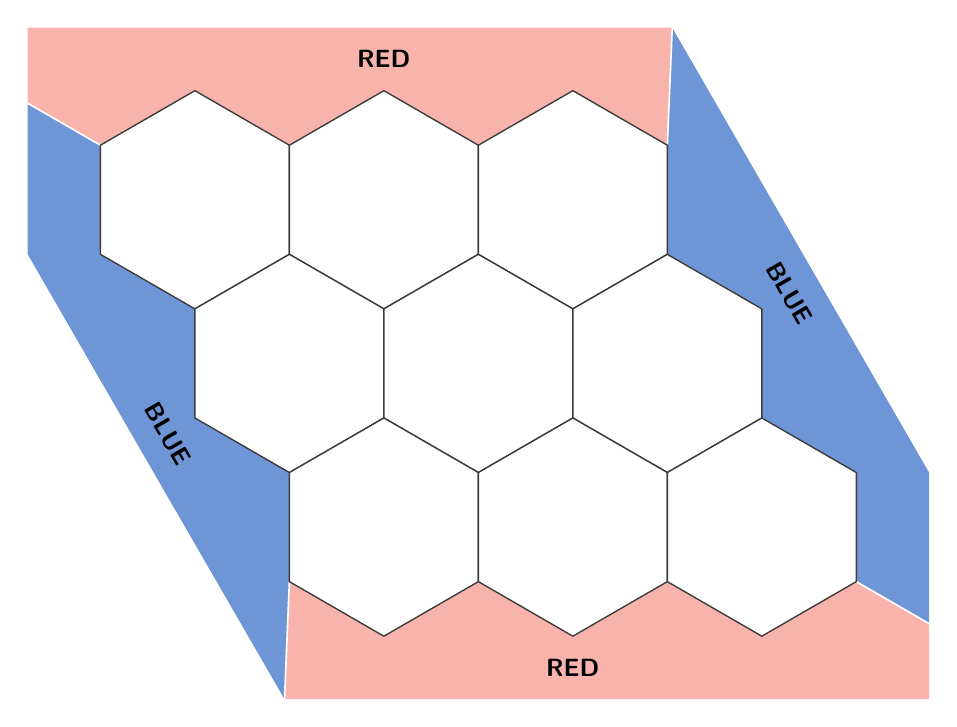
\begin{tikzpicture}[x=1.0mm,y=1.0mm,line join=round]
\begin{scope}
\clip (-21.238,-63.426) rectangle (93.238,21.856);
\fill[redtint] (-12.000,6.928) -- (0.000,13.856) -- (12.000,6.928) -- (24.000,13.856) -- (36.000,6.928) -- (48.000,13.856) -- (60.000,6.928) -- (60.619,21.856) -- (-37.856,21.856) -- cycle;
\fill[redtint] (84.000,-48.497) -- (72.000,-55.426) -- (60.000,-48.497) -- (48.000,-55.426) -- (36.000,-48.497) -- (24.000,-55.426) -- (12.000,-48.497) -- (11.381,-63.426) -- (109.856,-63.426) -- cycle;
\fill[bluetint] (12.000,-48.497) -- (12.000,-34.641) -- (0.000,-27.713) -- (-0.000,-13.856) -- (-12.000,-6.928) -- (-12.000,6.928) -- (-37.856,21.856) -- (11.381,-63.426) -- cycle;
\fill[bluetint] (60.000,6.928) -- (60.000,-6.928) -- (72.000,-13.856) -- (72.000,-27.713) -- (84.000,-34.641) -- (84.000,-48.497) -- (109.856,-63.426) -- (60.619,21.856) -- cycle;
\draw[white,line width=0.6pt] (-12.000,6.928) -- (-37.856,21.856);
\draw[white,line width=0.6pt] (60.000,6.928) -- (60.619,21.856);
\draw[white,line width=0.6pt] (84.000,-48.497) -- (109.856,-63.426);
\draw[white,line width=0.6pt] (12.000,-48.497) -- (11.381,-63.426);
\end{scope}
\node[font=\small\bfseries,text=black] at (24.000,17.856) {RED};
\node[font=\small\bfseries,text=black] at (48.000,-59.426) {RED};
\node[font=\small\bfseries,text=black,rotate=-60] at (-3.464,-29.713) {BLUE};
\node[font=\small\bfseries,text=black,rotate=-60] at (75.464,-11.856) {BLUE};
\filldraw[fill=white,draw=gridline,line width=0.5pt] (12.000,6.928) -- (0.000,13.856) -- (-12.000,6.928) -- (-12.000,-6.928) -- (-0.000,-13.856) -- (12.000,-6.928) -- cycle;
\filldraw[fill=white,draw=gridline,line width=0.5pt] (36.000,6.928) -- (24.000,13.856) -- (12.000,6.928) -- (12.000,-6.928) -- (24.000,-13.856) -- (36.000,-6.928) -- cycle;
\filldraw[fill=white,draw=gridline,line width=0.5pt] (60.000,6.928) -- (48.000,13.856) -- (36.000,6.928) -- (36.000,-6.928) -- (48.000,-13.856) -- (60.000,-6.928) -- cycle;
\filldraw[fill=white,draw=gridline,line width=0.5pt] (24.000,-13.856) -- (12.000,-6.928) -- (-0.000,-13.856) -- (0.000,-27.713) -- (12.000,-34.641) -- (24.000,-27.713) -- cycle;
\filldraw[fill=white,draw=gridline,line width=0.5pt] (48.000,-13.856) -- (36.000,-6.928) -- (24.000,-13.856) -- (24.000,-27.713) -- (36.000,-34.641) -- (48.000,-27.713) -- cycle;
\filldraw[fill=white,draw=gridline,line width=0.5pt] (72.000,-13.856) -- (60.000,-6.928) -- (48.000,-13.856) -- (48.000,-27.713) -- (60.000,-34.641) -- (72.000,-27.713) -- cycle;
\filldraw[fill=white,draw=gridline,line width=0.5pt] (36.000,-34.641) -- (24.000,-27.713) -- (12.000,-34.641) -- (12.000,-48.497) -- (24.000,-55.426) -- (36.000,-48.497) -- cycle;
\filldraw[fill=white,draw=gridline,line width=0.5pt] (60.000,-34.641) -- (48.000,-27.713) -- (36.000,-34.641) -- (36.000,-48.497) -- (48.000,-55.426) -- (60.000,-48.497) -- cycle;
\filldraw[fill=white,draw=gridline,line width=0.5pt] (84.000,-34.641) -- (72.000,-27.713) -- (60.000,-34.641) -- (60.000,-48.497) -- (72.000,-55.426) -- (84.000,-48.497) -- cycle;
\end{tikzpicture}
\end{center}
\vspace{8mm}

\prob{3} Can you put a red or a blue counter on every hexagon so that Red and Blue both win?
\begin{center}
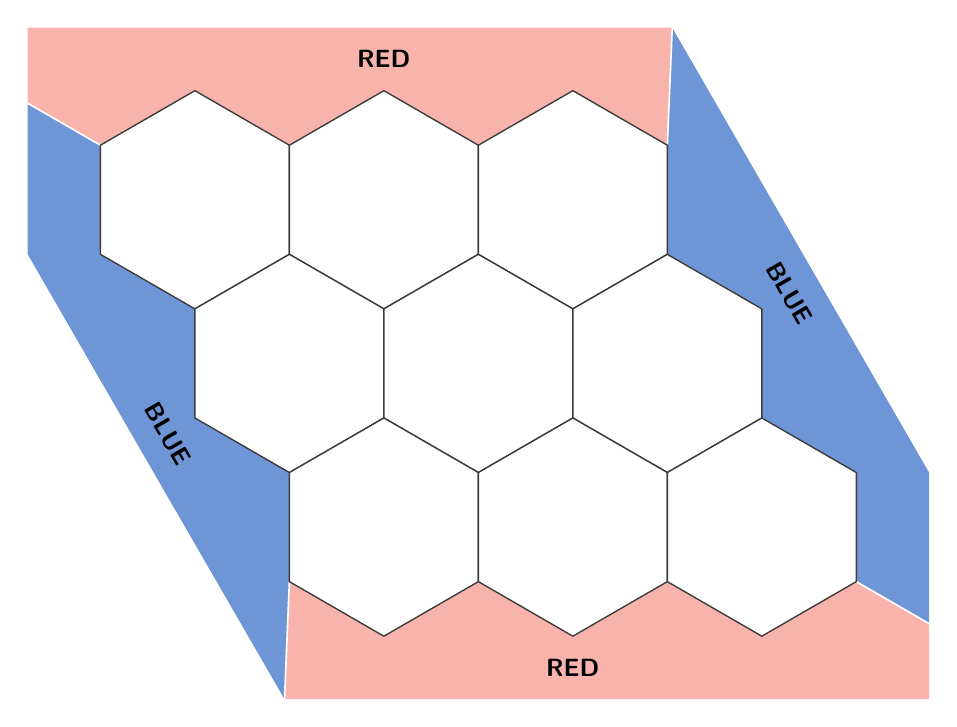
\begin{tikzpicture}[x=1.0mm,y=1.0mm,line join=round]
\begin{scope}
\clip (-21.238,-63.426) rectangle (93.238,21.856);
\fill[redtint] (-12.000,6.928) -- (0.000,13.856) -- (12.000,6.928) -- (24.000,13.856) -- (36.000,6.928) -- (48.000,13.856) -- (60.000,6.928) -- (60.619,21.856) -- (-37.856,21.856) -- cycle;
\fill[redtint] (84.000,-48.497) -- (72.000,-55.426) -- (60.000,-48.497) -- (48.000,-55.426) -- (36.000,-48.497) -- (24.000,-55.426) -- (12.000,-48.497) -- (11.381,-63.426) -- (109.856,-63.426) -- cycle;
\fill[bluetint] (12.000,-48.497) -- (12.000,-34.641) -- (0.000,-27.713) -- (-0.000,-13.856) -- (-12.000,-6.928) -- (-12.000,6.928) -- (-37.856,21.856) -- (11.381,-63.426) -- cycle;
\fill[bluetint] (60.000,6.928) -- (60.000,-6.928) -- (72.000,-13.856) -- (72.000,-27.713) -- (84.000,-34.641) -- (84.000,-48.497) -- (109.856,-63.426) -- (60.619,21.856) -- cycle;
\draw[white,line width=0.6pt] (-12.000,6.928) -- (-37.856,21.856);
\draw[white,line width=0.6pt] (60.000,6.928) -- (60.619,21.856);
\draw[white,line width=0.6pt] (84.000,-48.497) -- (109.856,-63.426);
\draw[white,line width=0.6pt] (12.000,-48.497) -- (11.381,-63.426);
\end{scope}
\node[font=\small\bfseries,text=black] at (24.000,17.856) {RED};
\node[font=\small\bfseries,text=black] at (48.000,-59.426) {RED};
\node[font=\small\bfseries,text=black,rotate=-60] at (-3.464,-29.713) {BLUE};
\node[font=\small\bfseries,text=black,rotate=-60] at (75.464,-11.856) {BLUE};
\filldraw[fill=white,draw=gridline,line width=0.5pt] (12.000,6.928) -- (0.000,13.856) -- (-12.000,6.928) -- (-12.000,-6.928) -- (-0.000,-13.856) -- (12.000,-6.928) -- cycle;
\filldraw[fill=white,draw=gridline,line width=0.5pt] (36.000,6.928) -- (24.000,13.856) -- (12.000,6.928) -- (12.000,-6.928) -- (24.000,-13.856) -- (36.000,-6.928) -- cycle;
\filldraw[fill=white,draw=gridline,line width=0.5pt] (60.000,6.928) -- (48.000,13.856) -- (36.000,6.928) -- (36.000,-6.928) -- (48.000,-13.856) -- (60.000,-6.928) -- cycle;
\filldraw[fill=white,draw=gridline,line width=0.5pt] (24.000,-13.856) -- (12.000,-6.928) -- (-0.000,-13.856) -- (0.000,-27.713) -- (12.000,-34.641) -- (24.000,-27.713) -- cycle;
\filldraw[fill=white,draw=gridline,line width=0.5pt] (48.000,-13.856) -- (36.000,-6.928) -- (24.000,-13.856) -- (24.000,-27.713) -- (36.000,-34.641) -- (48.000,-27.713) -- cycle;
\filldraw[fill=white,draw=gridline,line width=0.5pt] (72.000,-13.856) -- (60.000,-6.928) -- (48.000,-13.856) -- (48.000,-27.713) -- (60.000,-34.641) -- (72.000,-27.713) -- cycle;
\filldraw[fill=white,draw=gridline,line width=0.5pt] (36.000,-34.641) -- (24.000,-27.713) -- (12.000,-34.641) -- (12.000,-48.497) -- (24.000,-55.426) -- (36.000,-48.497) -- cycle;
\filldraw[fill=white,draw=gridline,line width=0.5pt] (60.000,-34.641) -- (48.000,-27.713) -- (36.000,-34.641) -- (36.000,-48.497) -- (48.000,-55.426) -- (60.000,-48.497) -- cycle;
\filldraw[fill=white,draw=gridline,line width=0.5pt] (84.000,-34.641) -- (72.000,-27.713) -- (60.000,-34.641) -- (60.000,-48.497) -- (72.000,-55.426) -- (84.000,-48.497) -- cycle;
\end{tikzpicture}
\end{center}

\clearpage
\prob{4} Play Hex on this bigger board.
\begin{center}
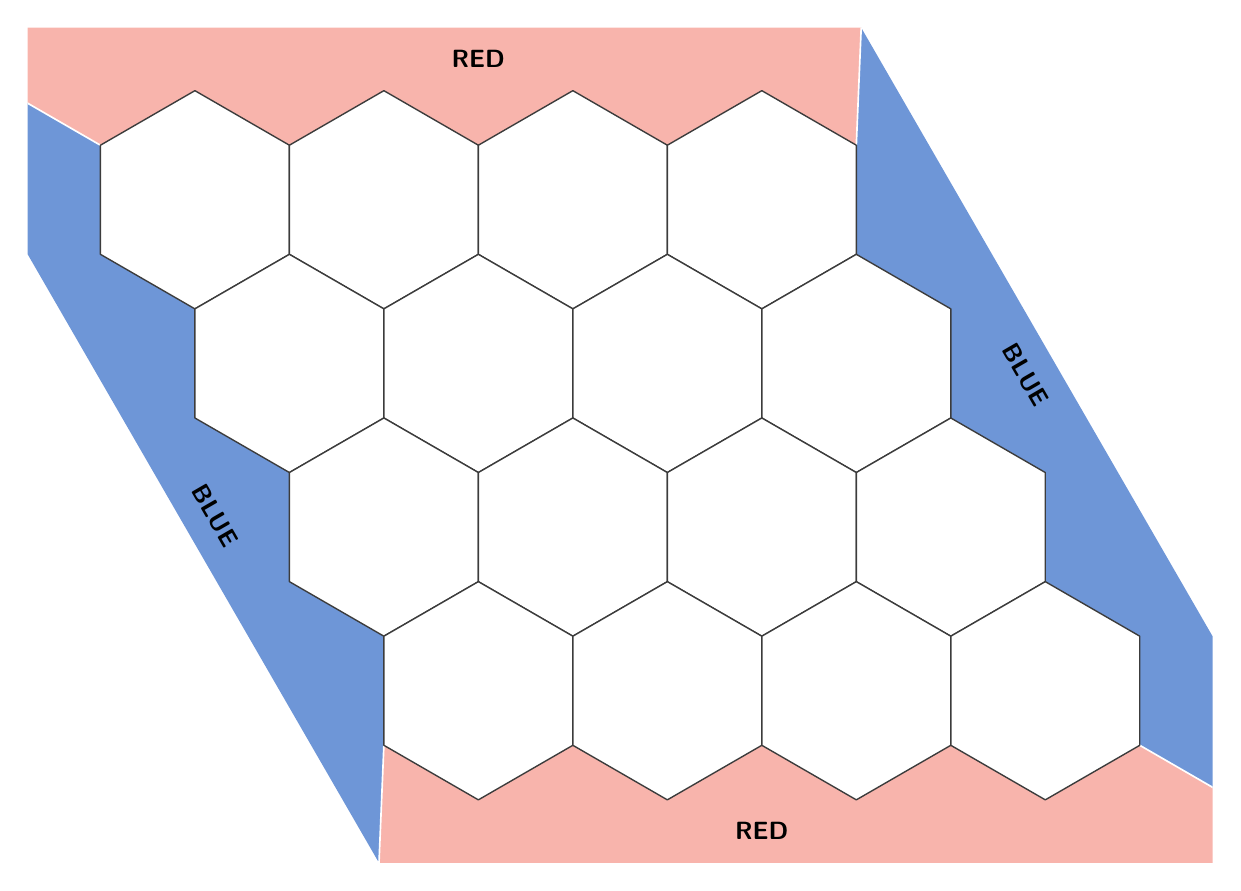
\begin{tikzpicture}[x=1.0mm,y=1.0mm,line join=round]
\begin{scope}
\clip (-21.238,-84.210) rectangle (129.238,21.856);
\fill[redtint] (-12.000,6.928) -- (0.000,13.856) -- (12.000,6.928) -- (24.000,13.856) -- (36.000,6.928) -- (48.000,13.856) -- (60.000,6.928) -- (72.000,13.856) -- (84.000,6.928) -- (84.619,21.856) -- (-37.856,21.856) -- cycle;
\fill[redtint] (120.000,-69.282) -- (108.000,-76.210) -- (96.000,-69.282) -- (84.000,-76.210) -- (72.000,-69.282) -- (60.000,-76.210) -- (48.000,-69.282) -- (36.000,-76.210) -- (24.000,-69.282) -- (23.381,-84.210) -- (145.856,-84.210) -- cycle;
\fill[bluetint] (24.000,-69.282) -- (24.000,-55.426) -- (12.000,-48.497) -- (12.000,-34.641) -- (0.000,-27.713) -- (-0.000,-13.856) -- (-12.000,-6.928) -- (-12.000,6.928) -- (-37.856,21.856) -- (23.381,-84.210) -- cycle;
\fill[bluetint] (84.000,6.928) -- (84.000,-6.928) -- (96.000,-13.856) -- (96.000,-27.713) -- (108.000,-34.641) -- (108.000,-48.497) -- (120.000,-55.426) -- (120.000,-69.282) -- (145.856,-84.210) -- (84.619,21.856) -- cycle;
\draw[white,line width=0.6pt] (-12.000,6.928) -- (-37.856,21.856);
\draw[white,line width=0.6pt] (84.000,6.928) -- (84.619,21.856);
\draw[white,line width=0.6pt] (120.000,-69.282) -- (145.856,-84.210);
\draw[white,line width=0.6pt] (24.000,-69.282) -- (23.381,-84.210);
\end{scope}
\node[font=\small\bfseries,text=black] at (36.000,17.856) {RED};
\node[font=\small\bfseries,text=black] at (72.000,-80.210) {RED};
\node[font=\small\bfseries,text=black,rotate=-60] at (2.536,-40.105) {BLUE};
\node[font=\small\bfseries,text=black,rotate=-60] at (105.464,-22.249) {BLUE};
\filldraw[fill=white,draw=gridline,line width=0.5pt] (12.000,6.928) -- (0.000,13.856) -- (-12.000,6.928) -- (-12.000,-6.928) -- (-0.000,-13.856) -- (12.000,-6.928) -- cycle;
\filldraw[fill=white,draw=gridline,line width=0.5pt] (36.000,6.928) -- (24.000,13.856) -- (12.000,6.928) -- (12.000,-6.928) -- (24.000,-13.856) -- (36.000,-6.928) -- cycle;
\filldraw[fill=white,draw=gridline,line width=0.5pt] (60.000,6.928) -- (48.000,13.856) -- (36.000,6.928) -- (36.000,-6.928) -- (48.000,-13.856) -- (60.000,-6.928) -- cycle;
\filldraw[fill=white,draw=gridline,line width=0.5pt] (84.000,6.928) -- (72.000,13.856) -- (60.000,6.928) -- (60.000,-6.928) -- (72.000,-13.856) -- (84.000,-6.928) -- cycle;
\filldraw[fill=white,draw=gridline,line width=0.5pt] (24.000,-13.856) -- (12.000,-6.928) -- (-0.000,-13.856) -- (0.000,-27.713) -- (12.000,-34.641) -- (24.000,-27.713) -- cycle;
\filldraw[fill=white,draw=gridline,line width=0.5pt] (48.000,-13.856) -- (36.000,-6.928) -- (24.000,-13.856) -- (24.000,-27.713) -- (36.000,-34.641) -- (48.000,-27.713) -- cycle;
\filldraw[fill=white,draw=gridline,line width=0.5pt] (72.000,-13.856) -- (60.000,-6.928) -- (48.000,-13.856) -- (48.000,-27.713) -- (60.000,-34.641) -- (72.000,-27.713) -- cycle;
\filldraw[fill=white,draw=gridline,line width=0.5pt] (96.000,-13.856) -- (84.000,-6.928) -- (72.000,-13.856) -- (72.000,-27.713) -- (84.000,-34.641) -- (96.000,-27.713) -- cycle;
\filldraw[fill=white,draw=gridline,line width=0.5pt] (36.000,-34.641) -- (24.000,-27.713) -- (12.000,-34.641) -- (12.000,-48.497) -- (24.000,-55.426) -- (36.000,-48.497) -- cycle;
\filldraw[fill=white,draw=gridline,line width=0.5pt] (60.000,-34.641) -- (48.000,-27.713) -- (36.000,-34.641) -- (36.000,-48.497) -- (48.000,-55.426) -- (60.000,-48.497) -- cycle;
\filldraw[fill=white,draw=gridline,line width=0.5pt] (84.000,-34.641) -- (72.000,-27.713) -- (60.000,-34.641) -- (60.000,-48.497) -- (72.000,-55.426) -- (84.000,-48.497) -- cycle;
\filldraw[fill=white,draw=gridline,line width=0.5pt] (108.000,-34.641) -- (96.000,-27.713) -- (84.000,-34.641) -- (84.000,-48.497) -- (96.000,-55.426) -- (108.000,-48.497) -- cycle;
\filldraw[fill=white,draw=gridline,line width=0.5pt] (48.000,-55.426) -- (36.000,-48.497) -- (24.000,-55.426) -- (24.000,-69.282) -- (36.000,-76.210) -- (48.000,-69.282) -- cycle;
\filldraw[fill=white,draw=gridline,line width=0.5pt] (72.000,-55.426) -- (60.000,-48.497) -- (48.000,-55.426) -- (48.000,-69.282) -- (60.000,-76.210) -- (72.000,-69.282) -- cycle;
\filldraw[fill=white,draw=gridline,line width=0.5pt] (96.000,-55.426) -- (84.000,-48.497) -- (72.000,-55.426) -- (72.000,-69.282) -- (84.000,-76.210) -- (96.000,-69.282) -- cycle;
\filldraw[fill=white,draw=gridline,line width=0.5pt] (120.000,-55.426) -- (108.000,-48.497) -- (96.000,-55.426) -- (96.000,-69.282) -- (108.000,-76.210) -- (120.000,-69.282) -- cycle;
\end{tikzpicture}
\end{center}

\clearpage
\prob{5} Can you put a red or a blue counter on every hexagon so that nobody wins?
\begin{center}
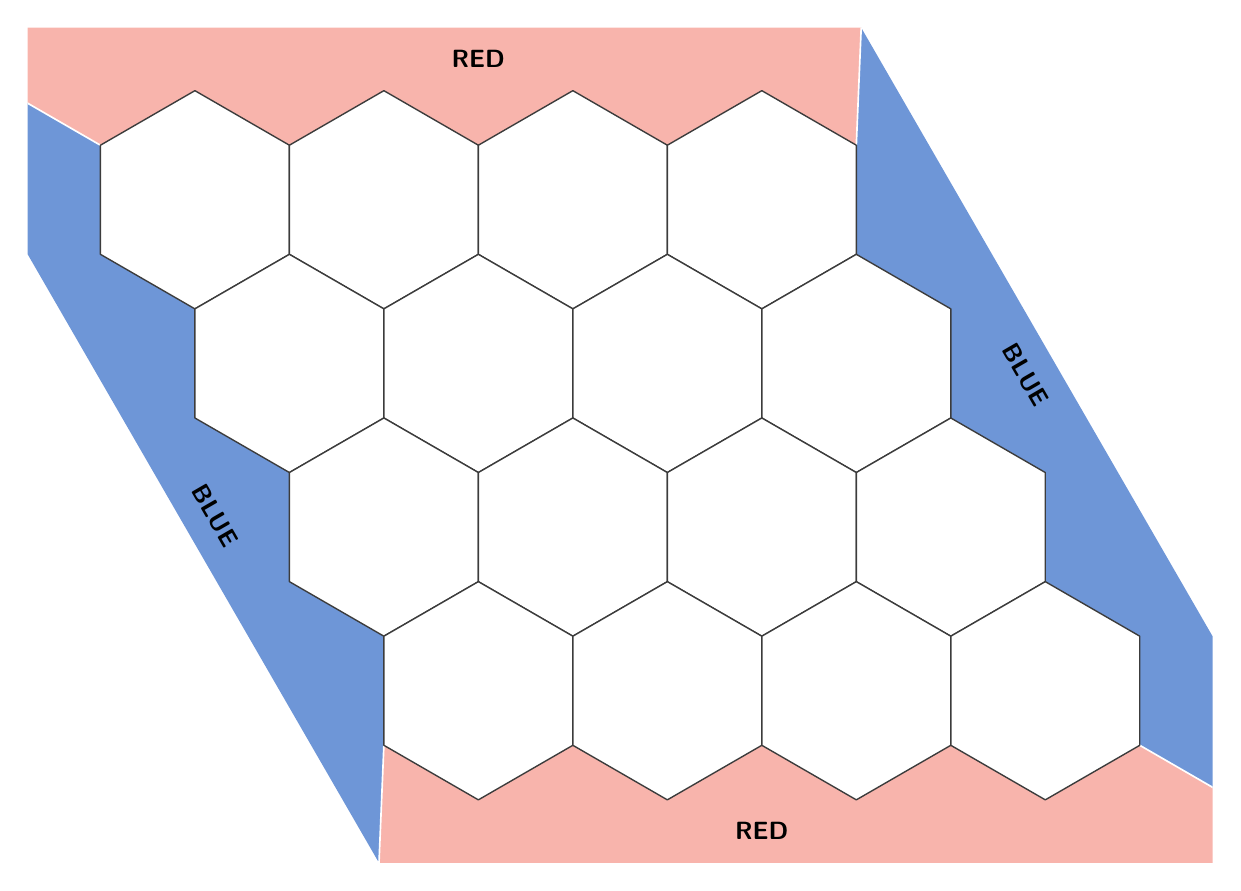
\begin{tikzpicture}[x=1.0mm,y=1.0mm,line join=round]
\begin{scope}
\clip (-21.238,-84.210) rectangle (129.238,21.856);
\fill[redtint] (-12.000,6.928) -- (0.000,13.856) -- (12.000,6.928) -- (24.000,13.856) -- (36.000,6.928) -- (48.000,13.856) -- (60.000,6.928) -- (72.000,13.856) -- (84.000,6.928) -- (84.619,21.856) -- (-37.856,21.856) -- cycle;
\fill[redtint] (120.000,-69.282) -- (108.000,-76.210) -- (96.000,-69.282) -- (84.000,-76.210) -- (72.000,-69.282) -- (60.000,-76.210) -- (48.000,-69.282) -- (36.000,-76.210) -- (24.000,-69.282) -- (23.381,-84.210) -- (145.856,-84.210) -- cycle;
\fill[bluetint] (24.000,-69.282) -- (24.000,-55.426) -- (12.000,-48.497) -- (12.000,-34.641) -- (0.000,-27.713) -- (-0.000,-13.856) -- (-12.000,-6.928) -- (-12.000,6.928) -- (-37.856,21.856) -- (23.381,-84.210) -- cycle;
\fill[bluetint] (84.000,6.928) -- (84.000,-6.928) -- (96.000,-13.856) -- (96.000,-27.713) -- (108.000,-34.641) -- (108.000,-48.497) -- (120.000,-55.426) -- (120.000,-69.282) -- (145.856,-84.210) -- (84.619,21.856) -- cycle;
\draw[white,line width=0.6pt] (-12.000,6.928) -- (-37.856,21.856);
\draw[white,line width=0.6pt] (84.000,6.928) -- (84.619,21.856);
\draw[white,line width=0.6pt] (120.000,-69.282) -- (145.856,-84.210);
\draw[white,line width=0.6pt] (24.000,-69.282) -- (23.381,-84.210);
\end{scope}
\node[font=\small\bfseries,text=black] at (36.000,17.856) {RED};
\node[font=\small\bfseries,text=black] at (72.000,-80.210) {RED};
\node[font=\small\bfseries,text=black,rotate=-60] at (2.536,-40.105) {BLUE};
\node[font=\small\bfseries,text=black,rotate=-60] at (105.464,-22.249) {BLUE};
\filldraw[fill=white,draw=gridline,line width=0.5pt] (12.000,6.928) -- (0.000,13.856) -- (-12.000,6.928) -- (-12.000,-6.928) -- (-0.000,-13.856) -- (12.000,-6.928) -- cycle;
\filldraw[fill=white,draw=gridline,line width=0.5pt] (36.000,6.928) -- (24.000,13.856) -- (12.000,6.928) -- (12.000,-6.928) -- (24.000,-13.856) -- (36.000,-6.928) -- cycle;
\filldraw[fill=white,draw=gridline,line width=0.5pt] (60.000,6.928) -- (48.000,13.856) -- (36.000,6.928) -- (36.000,-6.928) -- (48.000,-13.856) -- (60.000,-6.928) -- cycle;
\filldraw[fill=white,draw=gridline,line width=0.5pt] (84.000,6.928) -- (72.000,13.856) -- (60.000,6.928) -- (60.000,-6.928) -- (72.000,-13.856) -- (84.000,-6.928) -- cycle;
\filldraw[fill=white,draw=gridline,line width=0.5pt] (24.000,-13.856) -- (12.000,-6.928) -- (-0.000,-13.856) -- (0.000,-27.713) -- (12.000,-34.641) -- (24.000,-27.713) -- cycle;
\filldraw[fill=white,draw=gridline,line width=0.5pt] (48.000,-13.856) -- (36.000,-6.928) -- (24.000,-13.856) -- (24.000,-27.713) -- (36.000,-34.641) -- (48.000,-27.713) -- cycle;
\filldraw[fill=white,draw=gridline,line width=0.5pt] (72.000,-13.856) -- (60.000,-6.928) -- (48.000,-13.856) -- (48.000,-27.713) -- (60.000,-34.641) -- (72.000,-27.713) -- cycle;
\filldraw[fill=white,draw=gridline,line width=0.5pt] (96.000,-13.856) -- (84.000,-6.928) -- (72.000,-13.856) -- (72.000,-27.713) -- (84.000,-34.641) -- (96.000,-27.713) -- cycle;
\filldraw[fill=white,draw=gridline,line width=0.5pt] (36.000,-34.641) -- (24.000,-27.713) -- (12.000,-34.641) -- (12.000,-48.497) -- (24.000,-55.426) -- (36.000,-48.497) -- cycle;
\filldraw[fill=white,draw=gridline,line width=0.5pt] (60.000,-34.641) -- (48.000,-27.713) -- (36.000,-34.641) -- (36.000,-48.497) -- (48.000,-55.426) -- (60.000,-48.497) -- cycle;
\filldraw[fill=white,draw=gridline,line width=0.5pt] (84.000,-34.641) -- (72.000,-27.713) -- (60.000,-34.641) -- (60.000,-48.497) -- (72.000,-55.426) -- (84.000,-48.497) -- cycle;
\filldraw[fill=white,draw=gridline,line width=0.5pt] (108.000,-34.641) -- (96.000,-27.713) -- (84.000,-34.641) -- (84.000,-48.497) -- (96.000,-55.426) -- (108.000,-48.497) -- cycle;
\filldraw[fill=white,draw=gridline,line width=0.5pt] (48.000,-55.426) -- (36.000,-48.497) -- (24.000,-55.426) -- (24.000,-69.282) -- (36.000,-76.210) -- (48.000,-69.282) -- cycle;
\filldraw[fill=white,draw=gridline,line width=0.5pt] (72.000,-55.426) -- (60.000,-48.497) -- (48.000,-55.426) -- (48.000,-69.282) -- (60.000,-76.210) -- (72.000,-69.282) -- cycle;
\filldraw[fill=white,draw=gridline,line width=0.5pt] (96.000,-55.426) -- (84.000,-48.497) -- (72.000,-55.426) -- (72.000,-69.282) -- (84.000,-76.210) -- (96.000,-69.282) -- cycle;
\filldraw[fill=white,draw=gridline,line width=0.5pt] (120.000,-55.426) -- (108.000,-48.497) -- (96.000,-55.426) -- (96.000,-69.282) -- (108.000,-76.210) -- (120.000,-69.282) -- cycle;
\end{tikzpicture}
\end{center}

\clearpage
\prob{6} Red puts the first counter on the star. Can Red always win, whatever Blue does? Circle yes or no.
\begin{center}
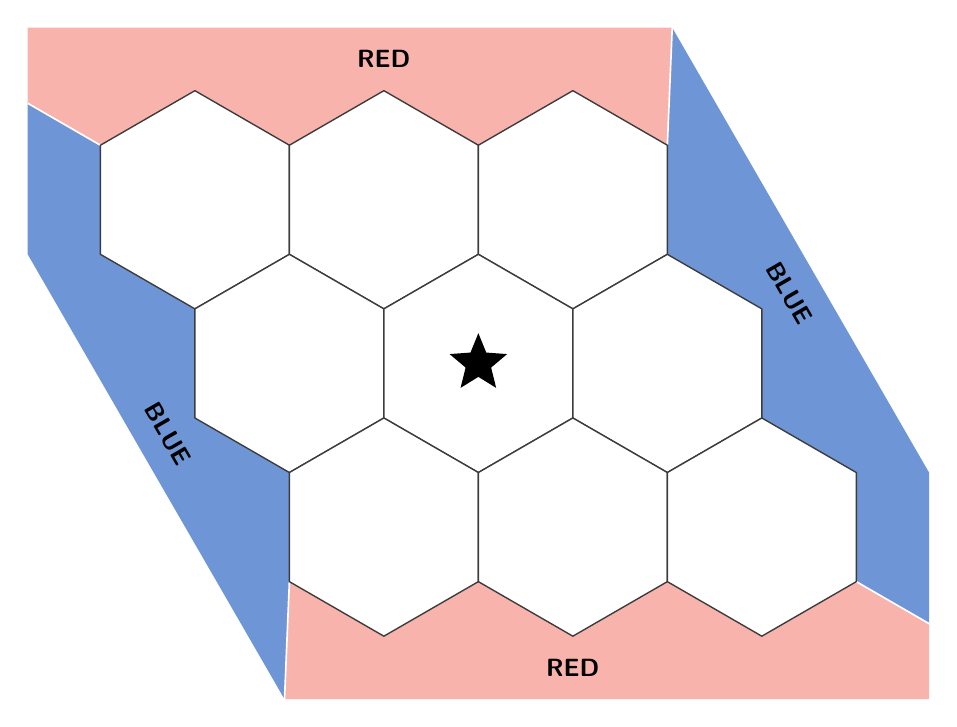
\begin{tikzpicture}[x=1.0mm,y=1.0mm,line join=round]
\begin{scope}
\clip (-21.238,-63.426) rectangle (93.238,21.856);
\fill[redtint] (-12.000,6.928) -- (0.000,13.856) -- (12.000,6.928) -- (24.000,13.856) -- (36.000,6.928) -- (48.000,13.856) -- (60.000,6.928) -- (60.619,21.856) -- (-37.856,21.856) -- cycle;
\fill[redtint] (84.000,-48.497) -- (72.000,-55.426) -- (60.000,-48.497) -- (48.000,-55.426) -- (36.000,-48.497) -- (24.000,-55.426) -- (12.000,-48.497) -- (11.381,-63.426) -- (109.856,-63.426) -- cycle;
\fill[bluetint] (12.000,-48.497) -- (12.000,-34.641) -- (0.000,-27.713) -- (-0.000,-13.856) -- (-12.000,-6.928) -- (-12.000,6.928) -- (-37.856,21.856) -- (11.381,-63.426) -- cycle;
\fill[bluetint] (60.000,6.928) -- (60.000,-6.928) -- (72.000,-13.856) -- (72.000,-27.713) -- (84.000,-34.641) -- (84.000,-48.497) -- (109.856,-63.426) -- (60.619,21.856) -- cycle;
\draw[white,line width=0.6pt] (-12.000,6.928) -- (-37.856,21.856);
\draw[white,line width=0.6pt] (60.000,6.928) -- (60.619,21.856);
\draw[white,line width=0.6pt] (84.000,-48.497) -- (109.856,-63.426);
\draw[white,line width=0.6pt] (12.000,-48.497) -- (11.381,-63.426);
\end{scope}
\node[font=\small\bfseries,text=black] at (24.000,17.856) {RED};
\node[font=\small\bfseries,text=black] at (48.000,-59.426) {RED};
\node[font=\small\bfseries,text=black,rotate=-60] at (-3.464,-29.713) {BLUE};
\node[font=\small\bfseries,text=black,rotate=-60] at (75.464,-11.856) {BLUE};
\filldraw[fill=white,draw=gridline,line width=0.5pt] (12.000,6.928) -- (0.000,13.856) -- (-12.000,6.928) -- (-12.000,-6.928) -- (-0.000,-13.856) -- (12.000,-6.928) -- cycle;
\filldraw[fill=white,draw=gridline,line width=0.5pt] (36.000,6.928) -- (24.000,13.856) -- (12.000,6.928) -- (12.000,-6.928) -- (24.000,-13.856) -- (36.000,-6.928) -- cycle;
\filldraw[fill=white,draw=gridline,line width=0.5pt] (60.000,6.928) -- (48.000,13.856) -- (36.000,6.928) -- (36.000,-6.928) -- (48.000,-13.856) -- (60.000,-6.928) -- cycle;
\filldraw[fill=white,draw=gridline,line width=0.5pt] (24.000,-13.856) -- (12.000,-6.928) -- (-0.000,-13.856) -- (0.000,-27.713) -- (12.000,-34.641) -- (24.000,-27.713) -- cycle;
\filldraw[fill=white,draw=gridline,line width=0.5pt] (48.000,-13.856) -- (36.000,-6.928) -- (24.000,-13.856) -- (24.000,-27.713) -- (36.000,-34.641) -- (48.000,-27.713) -- cycle;
\filldraw[fill=white,draw=gridline,line width=0.5pt] (72.000,-13.856) -- (60.000,-6.928) -- (48.000,-13.856) -- (48.000,-27.713) -- (60.000,-34.641) -- (72.000,-27.713) -- cycle;
\filldraw[fill=white,draw=gridline,line width=0.5pt] (36.000,-34.641) -- (24.000,-27.713) -- (12.000,-34.641) -- (12.000,-48.497) -- (24.000,-55.426) -- (36.000,-48.497) -- cycle;
\filldraw[fill=white,draw=gridline,line width=0.5pt] (60.000,-34.641) -- (48.000,-27.713) -- (36.000,-34.641) -- (36.000,-48.497) -- (48.000,-55.426) -- (60.000,-48.497) -- cycle;
\filldraw[fill=white,draw=gridline,line width=0.5pt] (84.000,-34.641) -- (72.000,-27.713) -- (60.000,-34.641) -- (60.000,-48.497) -- (72.000,-55.426) -- (84.000,-48.497) -- cycle;
\node[star,star points=5,star point ratio=2.25,fill=black,inner sep=0pt,minimum size=7.68mm] at (36.000,-20.785) {};
\end{tikzpicture}
\end{center}
\par\vspace{1mm}\centerline{\Large YES\hspace{36mm}NO}
\vspace{6mm}

\begin{center}
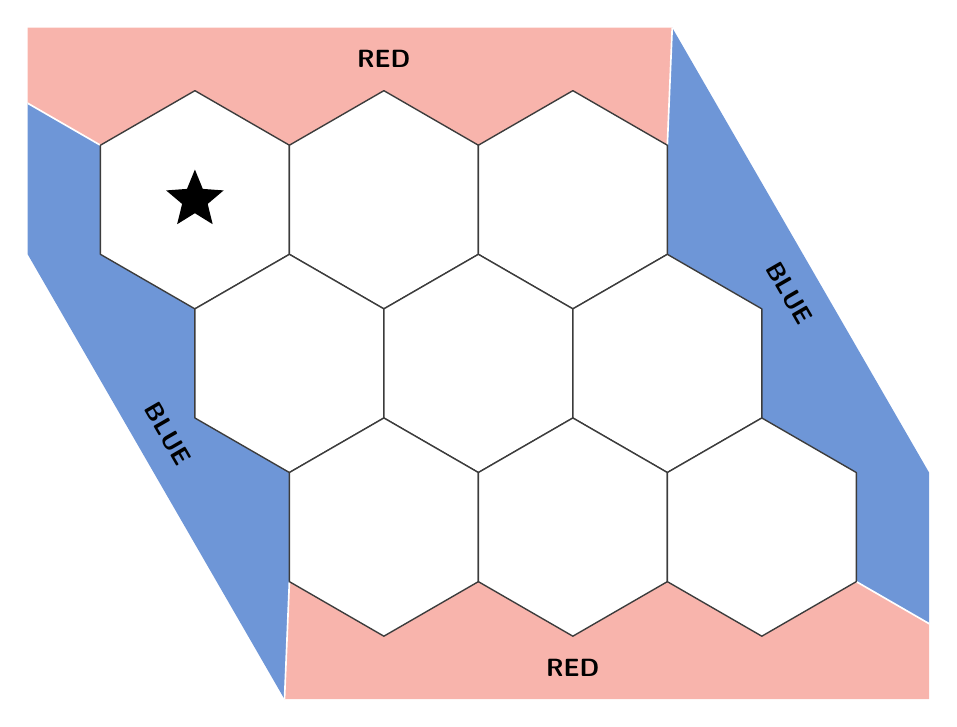
\begin{tikzpicture}[x=1.0mm,y=1.0mm,line join=round]
\begin{scope}
\clip (-21.238,-63.426) rectangle (93.238,21.856);
\fill[redtint] (-12.000,6.928) -- (0.000,13.856) -- (12.000,6.928) -- (24.000,13.856) -- (36.000,6.928) -- (48.000,13.856) -- (60.000,6.928) -- (60.619,21.856) -- (-37.856,21.856) -- cycle;
\fill[redtint] (84.000,-48.497) -- (72.000,-55.426) -- (60.000,-48.497) -- (48.000,-55.426) -- (36.000,-48.497) -- (24.000,-55.426) -- (12.000,-48.497) -- (11.381,-63.426) -- (109.856,-63.426) -- cycle;
\fill[bluetint] (12.000,-48.497) -- (12.000,-34.641) -- (0.000,-27.713) -- (-0.000,-13.856) -- (-12.000,-6.928) -- (-12.000,6.928) -- (-37.856,21.856) -- (11.381,-63.426) -- cycle;
\fill[bluetint] (60.000,6.928) -- (60.000,-6.928) -- (72.000,-13.856) -- (72.000,-27.713) -- (84.000,-34.641) -- (84.000,-48.497) -- (109.856,-63.426) -- (60.619,21.856) -- cycle;
\draw[white,line width=0.6pt] (-12.000,6.928) -- (-37.856,21.856);
\draw[white,line width=0.6pt] (60.000,6.928) -- (60.619,21.856);
\draw[white,line width=0.6pt] (84.000,-48.497) -- (109.856,-63.426);
\draw[white,line width=0.6pt] (12.000,-48.497) -- (11.381,-63.426);
\end{scope}
\node[font=\small\bfseries,text=black] at (24.000,17.856) {RED};
\node[font=\small\bfseries,text=black] at (48.000,-59.426) {RED};
\node[font=\small\bfseries,text=black,rotate=-60] at (-3.464,-29.713) {BLUE};
\node[font=\small\bfseries,text=black,rotate=-60] at (75.464,-11.856) {BLUE};
\filldraw[fill=white,draw=gridline,line width=0.5pt] (12.000,6.928) -- (0.000,13.856) -- (-12.000,6.928) -- (-12.000,-6.928) -- (-0.000,-13.856) -- (12.000,-6.928) -- cycle;
\filldraw[fill=white,draw=gridline,line width=0.5pt] (36.000,6.928) -- (24.000,13.856) -- (12.000,6.928) -- (12.000,-6.928) -- (24.000,-13.856) -- (36.000,-6.928) -- cycle;
\filldraw[fill=white,draw=gridline,line width=0.5pt] (60.000,6.928) -- (48.000,13.856) -- (36.000,6.928) -- (36.000,-6.928) -- (48.000,-13.856) -- (60.000,-6.928) -- cycle;
\filldraw[fill=white,draw=gridline,line width=0.5pt] (24.000,-13.856) -- (12.000,-6.928) -- (-0.000,-13.856) -- (0.000,-27.713) -- (12.000,-34.641) -- (24.000,-27.713) -- cycle;
\filldraw[fill=white,draw=gridline,line width=0.5pt] (48.000,-13.856) -- (36.000,-6.928) -- (24.000,-13.856) -- (24.000,-27.713) -- (36.000,-34.641) -- (48.000,-27.713) -- cycle;
\filldraw[fill=white,draw=gridline,line width=0.5pt] (72.000,-13.856) -- (60.000,-6.928) -- (48.000,-13.856) -- (48.000,-27.713) -- (60.000,-34.641) -- (72.000,-27.713) -- cycle;
\filldraw[fill=white,draw=gridline,line width=0.5pt] (36.000,-34.641) -- (24.000,-27.713) -- (12.000,-34.641) -- (12.000,-48.497) -- (24.000,-55.426) -- (36.000,-48.497) -- cycle;
\filldraw[fill=white,draw=gridline,line width=0.5pt] (60.000,-34.641) -- (48.000,-27.713) -- (36.000,-34.641) -- (36.000,-48.497) -- (48.000,-55.426) -- (60.000,-48.497) -- cycle;
\filldraw[fill=white,draw=gridline,line width=0.5pt] (84.000,-34.641) -- (72.000,-27.713) -- (60.000,-34.641) -- (60.000,-48.497) -- (72.000,-55.426) -- (84.000,-48.497) -- cycle;
\node[star,star points=5,star point ratio=2.25,fill=black,inner sep=0pt,minimum size=7.68mm] at (0.000,0.000) {};
\end{tikzpicture}
\end{center}
\par\vspace{1mm}\centerline{\Large YES\hspace{36mm}NO}

\clearpage
\prob{7} Put some blue counters on each board, then fill every other hexagon with red counters. Use as few blue counters as you can so that Red does not win.
\begin{center}
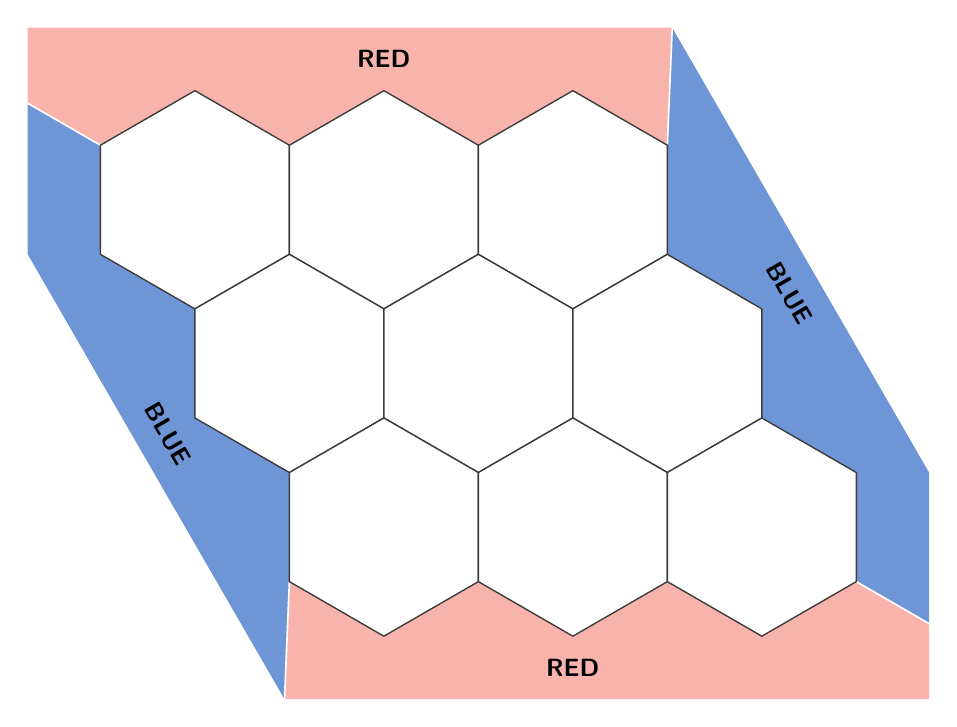
\begin{tikzpicture}[x=1.0mm,y=1.0mm,line join=round]
\begin{scope}
\clip (-21.238,-63.426) rectangle (93.238,21.856);
\fill[redtint] (-12.000,6.928) -- (0.000,13.856) -- (12.000,6.928) -- (24.000,13.856) -- (36.000,6.928) -- (48.000,13.856) -- (60.000,6.928) -- (60.619,21.856) -- (-37.856,21.856) -- cycle;
\fill[redtint] (84.000,-48.497) -- (72.000,-55.426) -- (60.000,-48.497) -- (48.000,-55.426) -- (36.000,-48.497) -- (24.000,-55.426) -- (12.000,-48.497) -- (11.381,-63.426) -- (109.856,-63.426) -- cycle;
\fill[bluetint] (12.000,-48.497) -- (12.000,-34.641) -- (0.000,-27.713) -- (-0.000,-13.856) -- (-12.000,-6.928) -- (-12.000,6.928) -- (-37.856,21.856) -- (11.381,-63.426) -- cycle;
\fill[bluetint] (60.000,6.928) -- (60.000,-6.928) -- (72.000,-13.856) -- (72.000,-27.713) -- (84.000,-34.641) -- (84.000,-48.497) -- (109.856,-63.426) -- (60.619,21.856) -- cycle;
\draw[white,line width=0.6pt] (-12.000,6.928) -- (-37.856,21.856);
\draw[white,line width=0.6pt] (60.000,6.928) -- (60.619,21.856);
\draw[white,line width=0.6pt] (84.000,-48.497) -- (109.856,-63.426);
\draw[white,line width=0.6pt] (12.000,-48.497) -- (11.381,-63.426);
\end{scope}
\node[font=\small\bfseries,text=black] at (24.000,17.856) {RED};
\node[font=\small\bfseries,text=black] at (48.000,-59.426) {RED};
\node[font=\small\bfseries,text=black,rotate=-60] at (-3.464,-29.713) {BLUE};
\node[font=\small\bfseries,text=black,rotate=-60] at (75.464,-11.856) {BLUE};
\filldraw[fill=white,draw=gridline,line width=0.5pt] (12.000,6.928) -- (0.000,13.856) -- (-12.000,6.928) -- (-12.000,-6.928) -- (-0.000,-13.856) -- (12.000,-6.928) -- cycle;
\filldraw[fill=white,draw=gridline,line width=0.5pt] (36.000,6.928) -- (24.000,13.856) -- (12.000,6.928) -- (12.000,-6.928) -- (24.000,-13.856) -- (36.000,-6.928) -- cycle;
\filldraw[fill=white,draw=gridline,line width=0.5pt] (60.000,6.928) -- (48.000,13.856) -- (36.000,6.928) -- (36.000,-6.928) -- (48.000,-13.856) -- (60.000,-6.928) -- cycle;
\filldraw[fill=white,draw=gridline,line width=0.5pt] (24.000,-13.856) -- (12.000,-6.928) -- (-0.000,-13.856) -- (0.000,-27.713) -- (12.000,-34.641) -- (24.000,-27.713) -- cycle;
\filldraw[fill=white,draw=gridline,line width=0.5pt] (48.000,-13.856) -- (36.000,-6.928) -- (24.000,-13.856) -- (24.000,-27.713) -- (36.000,-34.641) -- (48.000,-27.713) -- cycle;
\filldraw[fill=white,draw=gridline,line width=0.5pt] (72.000,-13.856) -- (60.000,-6.928) -- (48.000,-13.856) -- (48.000,-27.713) -- (60.000,-34.641) -- (72.000,-27.713) -- cycle;
\filldraw[fill=white,draw=gridline,line width=0.5pt] (36.000,-34.641) -- (24.000,-27.713) -- (12.000,-34.641) -- (12.000,-48.497) -- (24.000,-55.426) -- (36.000,-48.497) -- cycle;
\filldraw[fill=white,draw=gridline,line width=0.5pt] (60.000,-34.641) -- (48.000,-27.713) -- (36.000,-34.641) -- (36.000,-48.497) -- (48.000,-55.426) -- (60.000,-48.497) -- cycle;
\filldraw[fill=white,draw=gridline,line width=0.5pt] (84.000,-34.641) -- (72.000,-27.713) -- (60.000,-34.641) -- (60.000,-48.497) -- (72.000,-55.426) -- (84.000,-48.497) -- cycle;
\end{tikzpicture}
\end{center}
\vspace{4mm}

\begin{center}
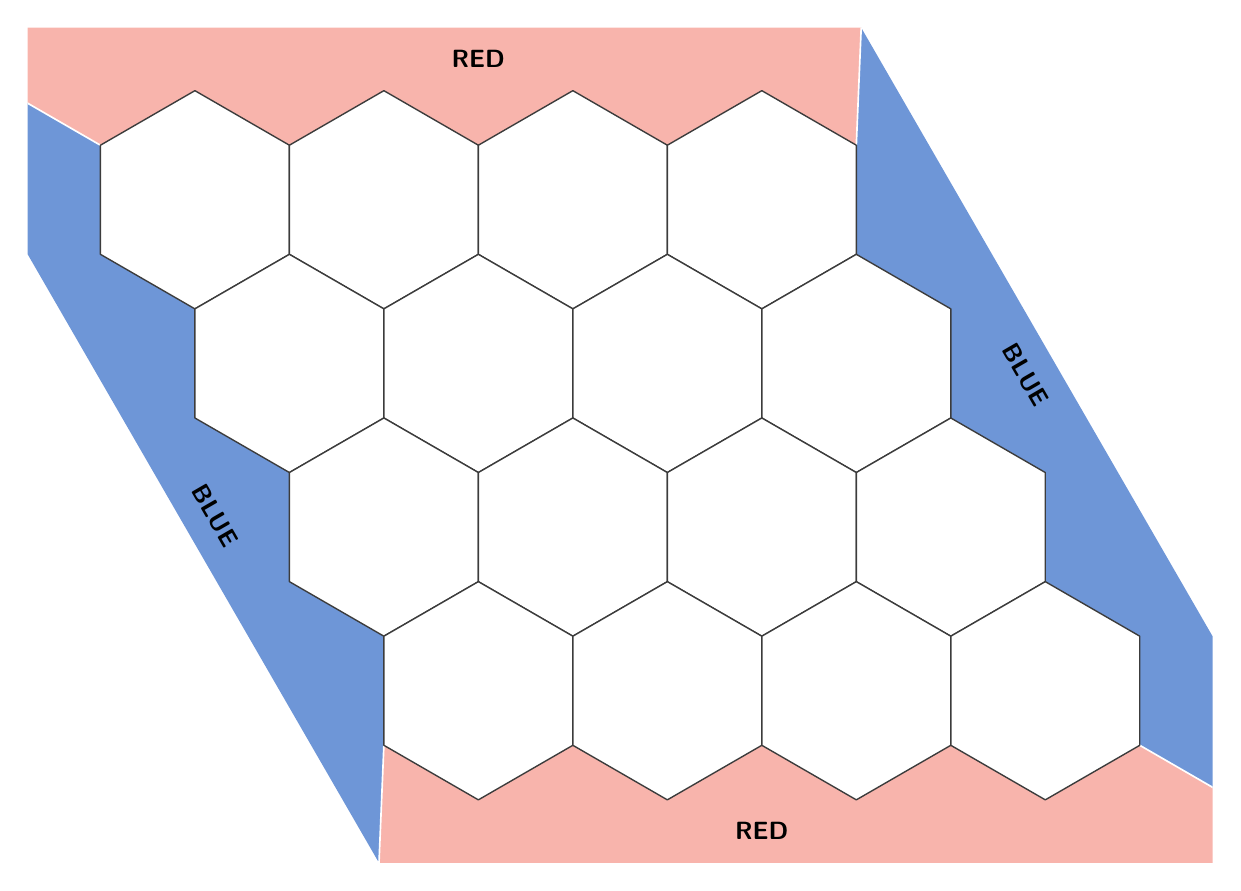
\begin{tikzpicture}[x=1.0mm,y=1.0mm,line join=round]
\begin{scope}
\clip (-21.238,-84.210) rectangle (129.238,21.856);
\fill[redtint] (-12.000,6.928) -- (0.000,13.856) -- (12.000,6.928) -- (24.000,13.856) -- (36.000,6.928) -- (48.000,13.856) -- (60.000,6.928) -- (72.000,13.856) -- (84.000,6.928) -- (84.619,21.856) -- (-37.856,21.856) -- cycle;
\fill[redtint] (120.000,-69.282) -- (108.000,-76.210) -- (96.000,-69.282) -- (84.000,-76.210) -- (72.000,-69.282) -- (60.000,-76.210) -- (48.000,-69.282) -- (36.000,-76.210) -- (24.000,-69.282) -- (23.381,-84.210) -- (145.856,-84.210) -- cycle;
\fill[bluetint] (24.000,-69.282) -- (24.000,-55.426) -- (12.000,-48.497) -- (12.000,-34.641) -- (0.000,-27.713) -- (-0.000,-13.856) -- (-12.000,-6.928) -- (-12.000,6.928) -- (-37.856,21.856) -- (23.381,-84.210) -- cycle;
\fill[bluetint] (84.000,6.928) -- (84.000,-6.928) -- (96.000,-13.856) -- (96.000,-27.713) -- (108.000,-34.641) -- (108.000,-48.497) -- (120.000,-55.426) -- (120.000,-69.282) -- (145.856,-84.210) -- (84.619,21.856) -- cycle;
\draw[white,line width=0.6pt] (-12.000,6.928) -- (-37.856,21.856);
\draw[white,line width=0.6pt] (84.000,6.928) -- (84.619,21.856);
\draw[white,line width=0.6pt] (120.000,-69.282) -- (145.856,-84.210);
\draw[white,line width=0.6pt] (24.000,-69.282) -- (23.381,-84.210);
\end{scope}
\node[font=\small\bfseries,text=black] at (36.000,17.856) {RED};
\node[font=\small\bfseries,text=black] at (72.000,-80.210) {RED};
\node[font=\small\bfseries,text=black,rotate=-60] at (2.536,-40.105) {BLUE};
\node[font=\small\bfseries,text=black,rotate=-60] at (105.464,-22.249) {BLUE};
\filldraw[fill=white,draw=gridline,line width=0.5pt] (12.000,6.928) -- (0.000,13.856) -- (-12.000,6.928) -- (-12.000,-6.928) -- (-0.000,-13.856) -- (12.000,-6.928) -- cycle;
\filldraw[fill=white,draw=gridline,line width=0.5pt] (36.000,6.928) -- (24.000,13.856) -- (12.000,6.928) -- (12.000,-6.928) -- (24.000,-13.856) -- (36.000,-6.928) -- cycle;
\filldraw[fill=white,draw=gridline,line width=0.5pt] (60.000,6.928) -- (48.000,13.856) -- (36.000,6.928) -- (36.000,-6.928) -- (48.000,-13.856) -- (60.000,-6.928) -- cycle;
\filldraw[fill=white,draw=gridline,line width=0.5pt] (84.000,6.928) -- (72.000,13.856) -- (60.000,6.928) -- (60.000,-6.928) -- (72.000,-13.856) -- (84.000,-6.928) -- cycle;
\filldraw[fill=white,draw=gridline,line width=0.5pt] (24.000,-13.856) -- (12.000,-6.928) -- (-0.000,-13.856) -- (0.000,-27.713) -- (12.000,-34.641) -- (24.000,-27.713) -- cycle;
\filldraw[fill=white,draw=gridline,line width=0.5pt] (48.000,-13.856) -- (36.000,-6.928) -- (24.000,-13.856) -- (24.000,-27.713) -- (36.000,-34.641) -- (48.000,-27.713) -- cycle;
\filldraw[fill=white,draw=gridline,line width=0.5pt] (72.000,-13.856) -- (60.000,-6.928) -- (48.000,-13.856) -- (48.000,-27.713) -- (60.000,-34.641) -- (72.000,-27.713) -- cycle;
\filldraw[fill=white,draw=gridline,line width=0.5pt] (96.000,-13.856) -- (84.000,-6.928) -- (72.000,-13.856) -- (72.000,-27.713) -- (84.000,-34.641) -- (96.000,-27.713) -- cycle;
\filldraw[fill=white,draw=gridline,line width=0.5pt] (36.000,-34.641) -- (24.000,-27.713) -- (12.000,-34.641) -- (12.000,-48.497) -- (24.000,-55.426) -- (36.000,-48.497) -- cycle;
\filldraw[fill=white,draw=gridline,line width=0.5pt] (60.000,-34.641) -- (48.000,-27.713) -- (36.000,-34.641) -- (36.000,-48.497) -- (48.000,-55.426) -- (60.000,-48.497) -- cycle;
\filldraw[fill=white,draw=gridline,line width=0.5pt] (84.000,-34.641) -- (72.000,-27.713) -- (60.000,-34.641) -- (60.000,-48.497) -- (72.000,-55.426) -- (84.000,-48.497) -- cycle;
\filldraw[fill=white,draw=gridline,line width=0.5pt] (108.000,-34.641) -- (96.000,-27.713) -- (84.000,-34.641) -- (84.000,-48.497) -- (96.000,-55.426) -- (108.000,-48.497) -- cycle;
\filldraw[fill=white,draw=gridline,line width=0.5pt] (48.000,-55.426) -- (36.000,-48.497) -- (24.000,-55.426) -- (24.000,-69.282) -- (36.000,-76.210) -- (48.000,-69.282) -- cycle;
\filldraw[fill=white,draw=gridline,line width=0.5pt] (72.000,-55.426) -- (60.000,-48.497) -- (48.000,-55.426) -- (48.000,-69.282) -- (60.000,-76.210) -- (72.000,-69.282) -- cycle;
\filldraw[fill=white,draw=gridline,line width=0.5pt] (96.000,-55.426) -- (84.000,-48.497) -- (72.000,-55.426) -- (72.000,-69.282) -- (84.000,-76.210) -- (96.000,-69.282) -- cycle;
\filldraw[fill=white,draw=gridline,line width=0.5pt] (120.000,-55.426) -- (108.000,-48.497) -- (96.000,-55.426) -- (96.000,-69.282) -- (108.000,-76.210) -- (120.000,-69.282) -- cycle;
\end{tikzpicture}
\end{center}

\end{document}
